\documentclass{article}
\usepackage[T1]{fontenc}

\usepackage{enumitem}
\usepackage{amssymb}

\usepackage[utf8]{inputenc}
\usepackage{lmodern}
\usepackage{longtable}
\usepackage{polski}
\usepackage[margin=2.5cm]{geometry}


\newcommand{\linia}{\rule{\linewidth}{0.4mm}}

\title{Komputerowe wspomaganie diagnozowania zawałów z wykorzystaniem algorytmu KNN}
\author{Bartosz Rodziewicz \hspace{.9cm} 226105\\ Kamil Dobrysiewicz \hspace{.8cm} 225961\\}
% Title page layout (fold)
\makeatletter
\renewcommand{\maketitle}{
\begin{titlepage}		

	\vspace{2cm}
		
	\begin{center}
		\begin{figure}[h]
			\centering
\includegraphics[width=4cm]{PWR}
			\label{fig:PWR}
		\end{figure}
	\end{center}	
	\centering\huge Politechnika Wrocławska\\
	\vspace{0.3cm}
	\centering\LARGE Wydział Elektroniki\\
	
	\vspace{2cm}
	
	\noindent\linia
	\begin{center}	
		\huge \textsc{Zastosowania Informatyki w Medycynie}\\
		\vspace{0.3cm}
		\LARGE \@title\\	
	\end{center}
	\linia

	\begin{center}
		\vspace{2cm}
		\textbf{\Large Autorzy:}\\
			\Large\@author \hspace{.3cm}
	\end{center}

	\begin{center}
		\vspace{2cm}	
		\textbf{\Large Prowadzący:}\\
		\Large Dr inż. Paweł Ksieniewicz\\
	\end{center}

	\end{titlepage}%
}
\makeatother
\usepackage{natbib}
\usepackage{graphicx}

\begin{document}

\maketitle

\tableofcontents

\newpage

\section{Założenia projektowe}
Celem niniejszego projektu jest nabycie umiejętności zastosowania algorytmu klasyfikacji nadzorowanej (w przypadku tego projektu algorytmu KNN) w zadaniu diagnozowania zawałów. Wymaga to odpowiedniej selekcji cech. Dostępność danych rzeczywistych umożliwi w przyszłości eksperymentalną ocenę skuteczności algorytmu i sprawdzenie, w jaki sposób jakość klasyfikacji zależy od liczby atrybutów wykorzystanych do skonstruowania modelu.

Wyróżniono następujące etapy realizacji projektu:
\begin{enumerate}
    \item Zapoznanie się z aglorytmem klasyfikacji, określonym w temacie projektu.
    \item Zapoznanie się z materiałem empirycznym - analiza danych wejściowych, określenie liczby i znaczenia klas oraz dokonanie charakterystyki cech.
    \item Opracowanie sposobu wyznaczania rankingu cech w wykorzystaniem rozwiązań dostępnych w bibliotece \texttt{scikit-learn}.
    \item Zaplanowanie badań eksperymentalnych.
    \item Implementacja algorytmu klasyfikacji.
    \item Przeprowadzenie badań eksperymentalnych.
    \item Analiza wyników i wyciągnięcie wniosków.
    \item Przygotowanie kompletnej dokumentacji.
\end{enumerate}{}

\newpage

\section{Charakterystyka analizowanego problemu}
Do badań wykorzystane będą dane dostarczone przez prowadzącego, zawierające 901 obiektów. Podzielono je na pięć plików, reprezentujących dostępne w badaniach diagnozy:
\begin{itemize}{}
    \item dusznicę bolesną,
    \item dusznicę odmienną (Prinzmetala),
    \item zawał mięśnia sercowego (pełnościenny),
    \item zawał mięśnia sercowego (podwsierdziowy),
    \item ból nie związany z sercem.
\end{itemize}

\noindent
W każdym z zestawów danych znajdują się informacje o obiektach opisanych za pomocą 59 cech, oznaczających wyniki badań pojedyńczego pacjenta. Cechy podzielono na 8 grup, które opisują:
\begin{itemize}
    \item dane o wieku i płci pacjenta,
    \item informacje o bólu, który wystąpił u chorego (lokalizacja, promieniowanie, charakter bólu, czas trwania ostatniego wystąpienia bólu),
    \item inne symptomy, które wystąpiły razem z bólem (nudności, pocenie się, odbijanie),
    \item historię wystąpień podobnego bólu (bóle związane z zawałem, dusznicą bolesną, powiązane z sercem),
    \item historię chorób pacjenta (występowanie zawałów w przeszłości, przewlekła niewydolnośc serca, nadciśnienie),
    \item informacje o obecnie zażywanych lekach (beta blokery, diuretyki, niesteroidowe leki przeciwzapalne),
    \item wyniki badania fizykalnego (ciśnienie krwi, tętno, sinica, szmery oddechowe),
    \item wyniki badania elektrokardiografem (EKG).
\end{itemize}{}
Większość cech ma charakter binarny, czyli posiada tylko dwie wartości (0 lub 1), np. płeć, czy pacjent zażywa beta blokery, czy chory ma nadciśnienie. Jest to najprostsza odmiana atrybutu kategorycznego. W zbiorze cech znaleźć można też kilka cech kategorycznych, które przyjmować mogą kilka wartości z grupy możliwych opcji, np. lokalizacja bólu, moment wystąpienia bólu, jego charakter, czy kierunek promieniowania. Wyróżnić można także cechy ciągłe, takie jak: wiek pacjenta, liczba godzin od rozpoczęcia bólu, ciśnienie skurczowe, tętno.

\newpage

\section{Opis zastosowanych algorytmów}

\subsection{Metryki odległości}
W grupie algorytmów minimalno-odległościowych, do której należy algorytm k-NN istotną rolę odgrywa zastosowana metryka odległości, wg której mierzone są odległości pomiędzy badanymi punktami. Spośród metryk dostpęnych w bibliotece \textit{scikit-learn} wybrano odległość Euklidesową oraz metrykę miejską (zwaną inaczej odległością Manhattan).

\subsubsection{Odległość Euklidesowa}
Odległość Euklidesowa stanowi jeden z najpopularniejszych sposobów obliczania odległości między obiektami w przestrzeni wielowymiarowej. Jej wartość obliczana jest za pomocą wzoru:\\
\begin{center}
    $d(A,B) = \sqrt{\sum_{i=1}^n(x_{Ai} - x_{Bi})^2}$
\end{center}{}
Odległość Euklidesowa jest więc równa długości odcinka, który łączy dwa dane punkty.

\subsubsection{Metryka miejska}
Metryka miejska to sposób obliczania odległości, gdzie możliwe jest poruszanie się tylko w dwóch prostopadłych do siebie kierunkach. Inna nazwa tej metryki to odległość Manhattan, ponieważ przypomina ona poruszanie się po ulicach Manhattanu. Jej wartość obliczana jest ze wzoru:\\
\begin{center}{}
    $d(A,B) = \sum_{i=1}^n|x_{Ai} - x_{Bi}|$
\end{center}

\newpage

\subsection{Algorytm K-NN}
Algrytm K-NN (k nearest neighbours - k najbliższych sąsiadów) jest jednym z nadzorowanych algorytmów uczenia maszynowego. Jego działanie opiera się na bardzo prostej idei przewidywania nieznanych wartości poprzez ich dopasowanie do najbardziej podobnych już znanych wartości. W przypadku poszukiwania najbardziej podobnego rozwiązania uzyskujemy algorytm 1NN. Zazwyczaj warto jednak wziąć pod uwagę kilka lub kilkanaście podobnych rozwiązań i wybrać rozwiązanie najbardziej popularne w tym zbiorze. Podobieństwo jest w tym przypadku obliczane na podstawie metryki odległości, jaka została przez nas wybrana, na przykład wcześniej omówionej odległości Euklidesowej, czy metryki miejskiej.\\

Na rysunku \ref{fig:knn} zaprezentowany został prosty przykład problemu klasyfikacji przy pomocy algorytmu KNN. W przypadku, kiedy wartość k wynosi 5, niebieski okrąg reprezentujący niesklasyfikowany obiekt zostanie przyporządkowany do zbioru zielonych kwadratów (3 kwadraty w pobliżu, zaś tylko 2 trójkąty). Do podobnej klasyfikacji dojdzie w przypadku, gdy wartość k wyniesie 10. Wtedy obiekt testowy również zostanie uznany za zielony kwadrat, których w pobliżu niebieskiego okręgu znajdzie się 6.

\begin{figure}[h]
    \centering
    \noindent 
    \vspace{.2cm}
    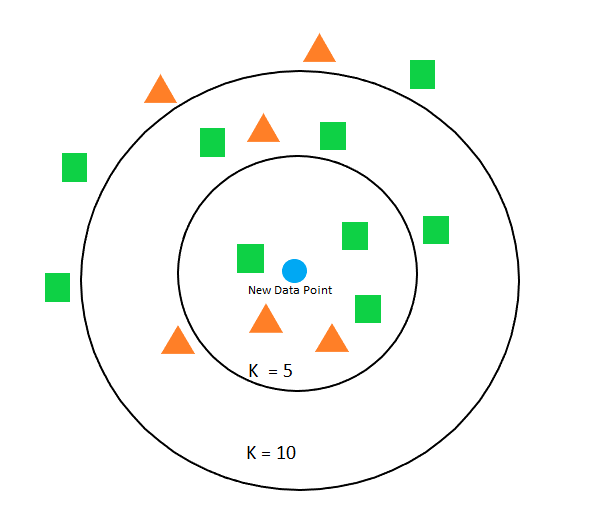
\includegraphics[width=10cm]{kNN.png}
    \caption{Przykład klasyfikacji przy pomocy algorytmu KNN.}
    \label{fig:knn}
\end{figure}

\newpage

\section{Stworzenie rankingu cech}
W niniejszym projekcie ranking cech wyznaczany był dla każdego zbioru testowego z osobna, ponieważ nie jest możliwe wyznaczenie jednego optymalnego rankingu cech dla całego zbioru danych.\\
Do stworzenia każdego z rankingów wykorzystano klasę \textbf{SelectKBest} z biblioteki scikit-learn. Algorytm filtrowania cech, jaki wykorzystano to $\chi^2$-distribution. Algorytm chi-squared został wybrany spośród dostępnych w bibliotece scikit-learn, ponieważ radzi sobie lepiej niż inne algorytmy z tej biblioteki ze zmiennymi nieciągłymi.\\
Metoda generująca ranking cech miała jednocześnie za zadanie usunięcie cech uznanych za nieistotne ze zbioru uczącego i testowego. Jako dane wejściowe przyjmuje zbiór danych uczących (osobno informacje o cechach i diagnozy) oraz liczbę najlepszych cech, które mają zostać wzięte pod uwagę w procesie klasyfikacji. Przebieg tej metody wygląda następująco:
\begin{enumerate}
    \item Stworzenie obiektu klasy \textbf{SelectKBest} z ustawieniem algorytmu filtrowania cech jako \textit{chi2} oraz liczby najlepszych cech, jakie mają zostać zwrócone (na podstawie parametru wejściowego metody).
    \item Wykonanie metody klasyfikującej dla zbioru uczącego.
    \item Pobranie identyfikatorów kolumn, zawierających najlepsze cechy.
    \item Eliminacja cech nieistotnych ze zbioru uczącego i testowego. Modyfikacja zbioru testowego została dokonana w celu zachowania spójności z zawartością zbioru uczącego.
\end{enumerate}
Metoda zwraca zredukowany zbiór uczący i testowy, na którym potem pracuje klasyfikator.\\

W tabeli \ref{tab:feature-ranking-table} przedstawiono zaś ranking cech, opracowany na początkowym etapie realizacji projektu, który został wyznaczony w oparciu o wszystkie dostępne obiekty.

\begin{center}
	\begin{longtable}{ |c|c|c| }
		\caption{25 najlepszych cech wg rankingu wyznaczonego dla wszystkich obiektów.}
		\label{tab:feature-ranking-table}\\
		\hline
			Numer cechy & Nazwa cechy & Wartość $\chi^2$ \\
		\hline
			35 & Systolic blood pressure & 1980.23 \\
			6 & Number of hours since onset & 978.58 \\
			2 & Pain location & 340.52 \\
			53 & New ST segment depression & 223.47 \\
			49 & New Q wave & 200.26 \\
			55 & New T wave inversion & 193.40 \\
			51 & New ST segment elevation & 188.22 \\
			54 & Any ST segment depression & 177.00 \\
			57 & New intraventricular conduction defect & 159.89 \\
			56 & Any T wave inversion & 151.67 \\
			38 & Respiration rate & 120.30 \\
			43 & Diastolic murmur & 117.16 \\
			58 & Any intraventricular conduction defect & 117.10 \\
			21 & Prior angina prectoris & 116.64 \\
			3 & Chest pain radiation & 114.72 \\
			37 & Heart rate & 109.56 \\
			50 & Any Q wave & 108.82 \\
			45 & S3 gallop & 105.09 \\
			17 & Prior pain related to heart & 101.63 \\
			18 & Prior pain due to MI & 89.17 \\
			46 & S4 gallop & 87.11 \\
			19 & Prior pain due to angina prectoris & 85.87 \\
			23 & Congestive heart failure & 85.27 \\
			42 & Systolic murmur & 84.50 \\
			25 & Hiatal hernia & 83.61 \\
		\hline
	\end{longtable}
\end{center}

\section{Implementacja klasyfikatora}
Samo wywołanie klasyfikatora nie okazało się bardzo wymagającym zadaniem, dzięki wykorzystaniu biblioteki scikit-learn, która oferuje bardzo szeroki wachlarz gotowych funkcjonalności w tym zakresie. Konieczne było jednak odpowiednie przygotowanie danych wejściowych dla klasyfikatora. Następnie przygotowano metodę, która przyjmuje na wejściu zbiór cech dostępnych obiektów badawczych, diagnozy dla tych zespołów cech, oraz zmienne istotne z punktu widzenia procesu badawczego, takie jak liczba sąsiadów, liczba najlepszych cech, jakie mają być brane pod uwagę w procesie klasyfikacji, czy wybrana metryka obliczania odległości między sąsiadami. W algorytmie zastosowano strategię dwóch powtórzeń pięciokrotnej walidacji krzyżowej. Podziału zbioru wejściowego na 5 części dokonano z wykorzystaniem klasy \textbf{StratifiedKFold}. Umożliwiła ona podział zbioru wejściowego na pięć podzbiorów, przy czym stosunek ilości obiektów zakwalifikowanych do poszczególnych klas jest dokładnie taki sam, jak dla całego zbioru przed podziałem. Przebieg metody wyznaczjącej skuteczność klasyfikatora wygląda następująco:
\begin{enumerate}
    \item Stworzenie obiektu klasy \textbf{StratifiedKFold} ze wskazaniem liczby grup, na jakie ma zostać podzielony zbiór danych wejściowych oraz ustawieniem zmiennej, która umożliwia jednakowe wyznaczenie grup dla wywołania głównej metody z innymi parametrami algorytmu.
    \item Dla każdego zestawu indeksów danych uczących i testowych zwróconego przez metodę \textit{split} klasy \textbf{StratifiedKFold} realizowane są kolejno następujące operacje:
        \begin{enumerate}
            \item Stworzenie dedykowanych zbiorów danych uczących i testowych (osobno zbiory cech i dedykowane im klasy) na podstawie ustalonych indeksów.
            \item Generacja zbioru cech uczących i testowych na podstawie rankingu cech wyznaczanego indywidualnie dla każdego zadania klasyfikacji.
            \item Stworzenie instancji klasyfikatora KNN z zadaną liczbą sąsiadów i wybraną metryką obliczania odległości.
            \item Dopasowanie modelu na podstawie danych uczących.
            \item Obliczenie skuteczności klasyfikacji danych testowych.
        \end{enumerate}
\end{enumerate}
Algorytm zwraca macierz złożoną z wyników działania klasyfikatora o liczbie kolumn równej liczbie warstw, na jakie został podzielony zbiór wejściowy.\\
Przykładowy wynik uruchomienia algorytmu przedstawiono na rysunku \ref{fig:knn_score}:

\begin{figure}[h]
    \centering
    \noindent 
    \vspace{.2cm}
    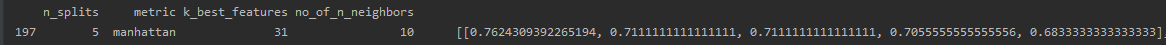
\includegraphics[width=16cm]{knn_score.png}
    \caption{Przykładowy wynik działania klasyfikatora.}
    \label{fig:knn_score}
\end{figure}

\section{Środowisko programistyczne}
Środowisko programistyczne stanowił edytor Atom uruchomiony w systemie Windows. Algorytm był testowany z poziomu systemu Ubuntu zainstalowanego przez Windows Subsystem for Linux w systemie Windows. Uruchomienie algorytmu powiodło się również z poziomu wiersza polecenia w Windows 10. W projekcie wykorzystano język Python w wersji 3 oraz biblioteki scikit-learn, pandas i numpy. Badania wykononane zostały na komputerze stacjonarnym wyposażonym w procesor Intel Core i5 czwartej generacji oraz 8GB pamięci operacyjnej.

\section{Opis badań eksperementalnych}
Przygotowany klasyfikator poddany został badaniom skuteczności działania. Zweryfikowano poprawność klasyfikacji dla następujących parametrów:
\begin{itemize}
    \item liczba sąsiadów - 1, 5, 10.
    \item metoda obliczania odległości między sąsiadami - odległość Euklidesowa i metryka miejska.
    \item liczba najlepszych cech w rankingu - od 1 do 35.
\end{itemize} 

Badania przeprowadzono dla liczby najlepszych cech z przedziału od 1 do 35, ponieważ przy liczbie 29 cech udało się uzyskać najlepsze rezultaty, potem wyniki były już gorsze. Dla każdej kombinacji parametrów wejściowych uzyskano uśrednione wyniki względem 5 powtórzeń metody 2-krotnej walidacji krzyżowej.

\section{Wyniki badań}
W wyniku przeprowadzonych badań skuteczności klasyfikatora KNN otrzymano 210 rezultatów dla różnych kombinacji parametrów omówionych w poprzedniej sekcji. Każdy z wyników został uśredniony względem 2 powtórzeń 5-krotnej walidacji krzyżowej. W tabeli \ref{tab:srednie_wyniki} przedstawiono ranking 25 najlepszych rezultatów, sporządzony na podstawie uśrednionych wyników działania klasyfikatora, zaokrąglonych do dwóch miejsc po przecinku.

\begin{center}
	\begin{longtable}{ |c|c|c|c|c| }
		\caption{25 najlepszych wyników działania klasyfikatora KNN.}
		\label{tab:srednie_wyniki}\\
		\hline
			Identyfikator testu & Metryka odległości & Liczba cech & Liczba sąsiadów & Skuteczność algorytmu (\%) \\
		\hline
            197 & Manhattan & 31 & 10 & 72,36\\
            203	& Manhattan & 33 & 10 & 72,25\\
            188	& Manhattan & 28 & 10 & 72,2\\
            205	& Manhattan & 34 & 5 & 72,19\\
            206	& Manhattan & 34 & 10 & 72,14\\
            209	& Manhattan & 35 & 10 & 72,09\\
            202 & Manhattan & 33 & 5 & 72,08\\
            190	& Manhattan & 29 & 5 & 71,75\\
            191	& Manhattan & 29 & 10 & 71,7\\
            193	& Manhattan & 30 & 5 & 71,64\\
            194	& Manhattan & 30 & 10 & 71,64\\
            208	& Manhattan & 35 & 5 & 71,53\\
            196	& Manhattan & 31 & 5 & 71,47\\
            199	& Manhattan & 32 & 5 & 71,42\\
            200	& Manhattan & 32 & 10 & 71,31\\
            178	& Manhattan & 25 & 5 & 71,25\\
            173	& Manhattan & 23 & 10 & 71,25\\
            176	& Manhattan & 24 & 10 & 71,2\\
            175	& Manhattan & 24 & 5 & 71,14\\
            170	& Manhattan & 22 & 10 & 70,87\\
            181	& Manhattan & 26 & 5 & 70,87\\
            179	& Manhattan & 25 & 10 & 70,86\\
            187	& Manhattan & 28 & 5 & 70,7\\
            182	& Manhattan & 26 & 10 & 70,7\\
            172	& Manhattan & 23 & 5 & 70,64\\
		\hline
	\end{longtable}
\end{center}

\newpage

Przedstawione rezultaty pozwalają na wyciągnięcie pewnych wniosków, jednak istnieje ryzyko, że niektóre z nich zostały zawyżone lub zaniżone poprzez wylosowanie sprzyjającego zbioru uczącego i testowego. W celu zwiększenia wiarygodności wyników postanowiono dokonać analizy statystycznej na zasadzie testów parowych ze skorygowanym testem t-Studenta dla powtórzonej walidacji krzyżowej.

\subsection{Skorygowany test t-Studenta dla powtórzonej walidacji krzyżowej}
W celu zwiększenia wiarygodności uzyskanych wyników dla każdej możliwej pary dwóch macierzy z wynikami działania algorytmu obliczona została statystyka na podstawie wzoru:
$$ t = \frac{\overline{S}}{\sqrt{(\frac{1}{J*k} + \frac{N_t_s}{N_t_r}})*\sum_{i=1}^k \sum_{j=1}^J \frac{(S^{(i,j)} - \overline{S})^2}{k*J-1}} \sim t_{k*J-1}, $$
gdzie \textit{J} stanowi liczbę powtórzeń (=2), \textit{k} - liczbę warstw (=5), \textit{S} - macierz różnicy wyników porównywanych testów, \textit{$\overline{S}$} - średnią wartość elementu macierzy \textit{S}, \textit{$S^{(i,j)}$} - pojedynczy wynik dla i-tej części (foldu) i J-tego powtórzenia. Wartość $\frac{N_{ts}}{N_{tr}}$ została uproszczona na potrzeby ninejszego projektu i wynosi $\frac{1}{k}$, czyli 0,2.\\
Obliczone wartości testu t-Studenta porównane zostały z wartością krytyczną z tablicy rozkładu t-Studenta. Wartość krytyczna wyniosła 2,2622 (poziom prawdopodobieństwa - 5\%, liczba stopni swobody - k * J - 1 = 9). Jeżeli wartość testu była większa niż wartość krytyczna to pierwszy wynik z pary uznawany był za statystycznie lepszy, jeżeli była mniejsza od ujemnej wartości krytycznej to drugi wynik uznawany był za lepszy, zaś jeżeli mieściła się w przedziale $<$ujemna wartość krytyczna; dodatnia wartość krytyczna$>$ to wyniki uznawane były za jednakowo wartościowe.

\subsection{Wyniki badań z uwzględnieniem rezultatów testów t-Studenta}
Rezultatem obliczeń wartości testu t-Studenta była macierz 210x210, której komórki zawierają liczby ze zbioru \{-1, 0, 1\}, oznaczające kolejno kolejno: -1 - rezultat testu o numerze równym numerowi wiersza jest statystycznie gorszy od rezultatu testu o numerze równym numerowi kolumny, 0 - porównywane testy są statycznie jednakowo dobre, 1 - rezultat o numerze równym numerowi wiersza jest statystycznie lepszy od rezultatu o numerze równym numerowi kolumny. Fragment tej macierzy przedstawiono na rysunku \ref{fig:macierz_210}:

\begin{figure}[h]
    \centering
    \noindent 
    \vspace{.2cm}
    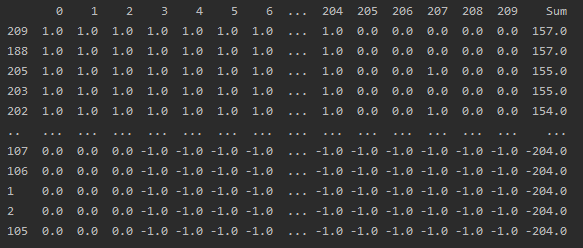
\includegraphics[width=14cm]{macierz_210.png}
    \caption{Fragment macierzy z interpretacją wyników testu t-Studenta.}
    \label{fig:macierz_210}
\end{figure}

\newpage

Wyniki zawarte w otrzymanej macierzy zostały zsumowane i na ich podstawie ponownie został wyznaczony ranking skuteczości działania klasyfikatora KNN. 25 najlepszych wyników prezentuje tabela \ref{tab:wyniki_po_t}.

\begin{center}
	\begin{longtable}{ |c|c|c|c|c| }
		\caption{25 najlepszych wyników działania klasyfikatora KNN z uwzględnieniem wyników testu t-Studenta.}
		\label{tab:wyniki_po_t}\\
		\hline
			Identyfikator testu & Metryka odległości & Liczba cech & Liczba sąsiadów & Skuteczność algorytmu (\%) \\
		\hline
            188 & Manhattan & 28 & 10 & 72,2\\
            209 & Manhattan & 35 & 10 & 72,09\\
            203 & Manhattan & 33 & 10 & 72,25\\
            205 & Manhattan & 34 & 5 & 72,19\\
            202 & Manhattan & 33 & 5 & 72,08\\
            191 & Manhattan & 29 & 10 & 71,7\\
            190 & Manhattan & 29 & 5 & 71,75\\
            194 & Manhattan & 30 & 10 & 71,64\\
            206 & Manhattan & 34 & 10 & 72,14\\
            196 & Manhattan & 31 & 5 & 71,47\\
            197 & Manhattan & 31 & 10 & 72,36\\
            193 & Manhattan & 30 & 5 & 71,64\\
            178 & Manhattan & 25 & 5 & 71,25\\
            175 & Manhattan & 24 & 5 & 71,14\\
            173 & Manhattan & 23 & 10 & 71,25\\
            176 & Manhattan & 24 & 10 & 71,2\\
            170 & Manhattan & 22 & 10 & 70,87\\
            208 & Manhattan & 35 & 5 & 71,53\\
            164 & Manhattan & 20 & 10 & 70,48\\
            199 & Manhattan & 32 & 5 & 71,42\\
            182 & Manhattan & 26 & 10 & 70,7\\
            158 & Manhattan & 18 & 10 & 70,2\\
            187 & Manhattan & 28 & 5 & 70,7\\
            166 & Manhattan & 21 & 5 & 70,36\\
            161 &Manhattan & 19 & 10 & 70,15\\
		\hline
	\end{longtable}
\end{center}

Dla najlepszego rezultatu wygenerowano przykładową macierz konfucji. Przedstawiono ją na rysunku \ref{fig:matrix}:

\begin{figure}[h]
    \centering
    \noindent 
    \vspace{.2cm}
    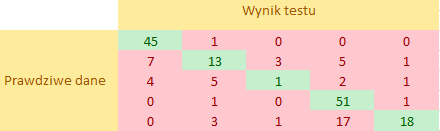
\includegraphics[width=12cm]{matrix.png}
    \caption{Macierz konfuzji dla statystycznie najlepszego zestawu parametrów wejściowych.}
    \label{fig:matrix}
\end{figure}

W macierzy konfuzji na zielono zaznaczono liczbę poprawnych przyporządkowań do danej klasy.
Na jej podstawie można wyciągnąć wniosek, że klasyfikator najczęściej mylił się, klasyfikując podwsierdziowy zawał mięśnia sercowego jako zawał pełnościenny (33\% przyporządkowań). Ponadto algorytm miał problem z diagnozowaniem dusznicy odmiennej. Było to prawdopodobnie spowodowane małą liczbą danych wejściowych dotyczących tej choroby.

\newpage

Na podstawie otrzymanych wyników można wyciągnąć wniosek, że dla badanego problemu lepszą metryką obliczania odległości między sąsiadami jest miara Manhattan. Wszystkie najlepsze wyniki uzyskane zostały właśnie dla tej metryki. Potwierdza to dodatkowo wykres najlepszych wyników dla obu miar odległości przedstawiony na rysunku \ref{fig:metryki}:

\begin{figure}[h]
    \centering
    \noindent 
    \vspace{.2cm}
    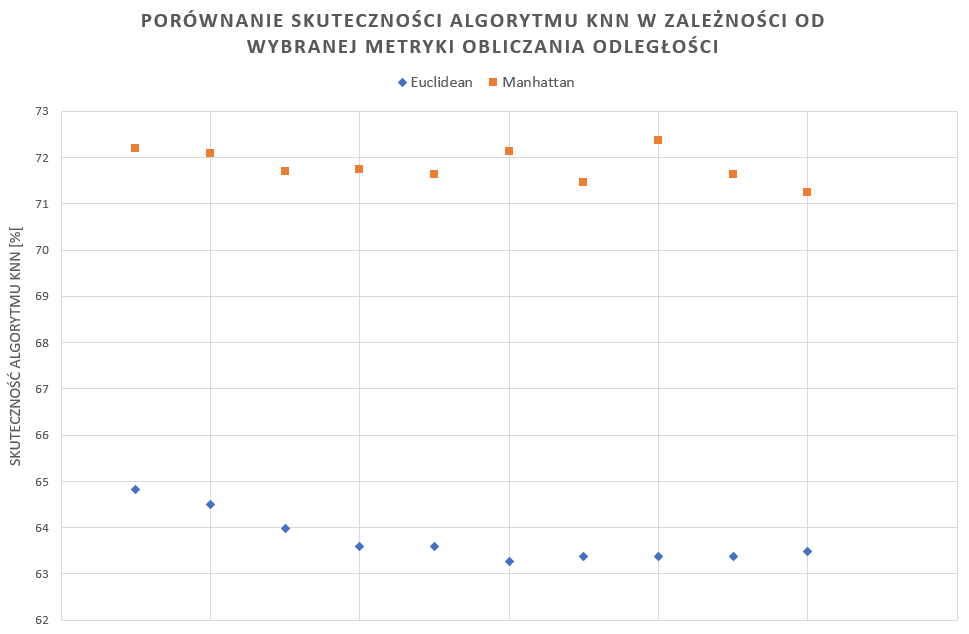
\includegraphics[width=16cm]{metryki.png}
    \caption{Porównanie najlepszych wyników klasyfikatora KNN w zależności od metryki wyznaczania odległości.}
    \label{fig:metryki}
\end{figure}
\noindent
Z rysunku \ref{fig:metryki} można ponadto odczytać, że metryka miejska pozwoliła na uzyskanie wyników o ok. 8\% lepszych od metryki euklidesowej.\\

\newpage

Kolejny wykres przedstawia zależność wyników od liczby cech branych pod uwagę w procesie klasyfikacji.

\begin{figure}[h]
    \centering
    \noindent 
    \vspace{.2cm}
    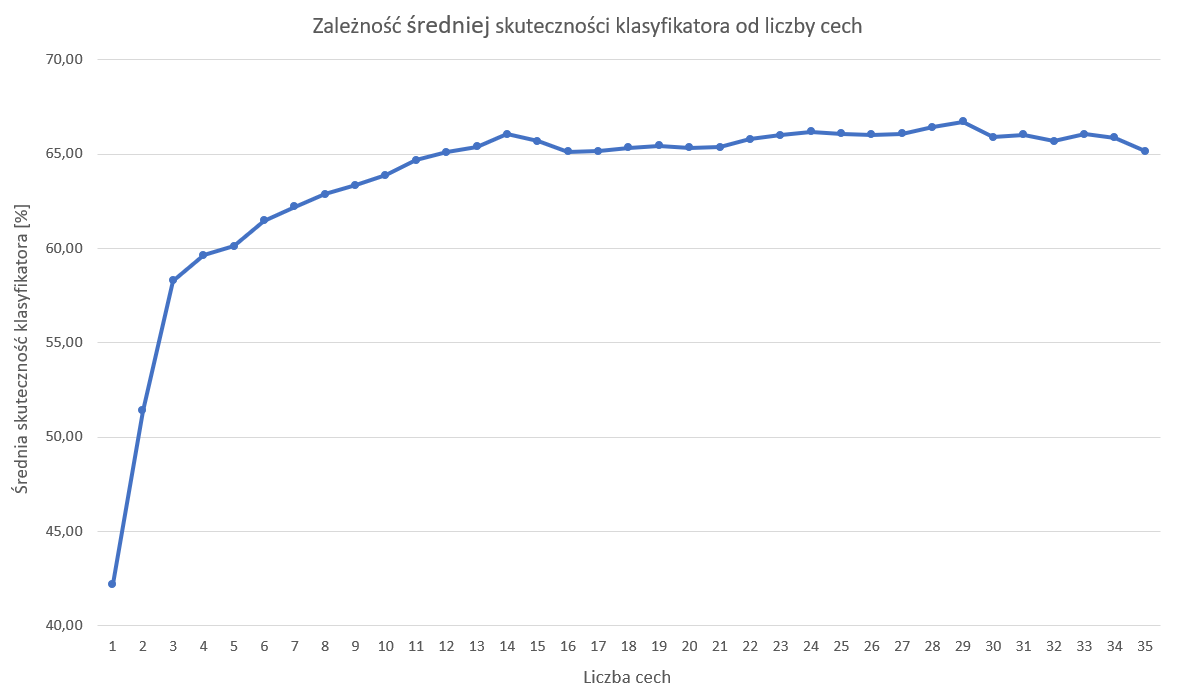
\includegraphics[width=16cm]{Cechy.png}
    \caption{Wykres zależności wyników klasyfikacji od liczby cech branych pod uwagę.}
    \label{fig:cechy}
\end{figure}

\noindent
Na podstawie wykresu przedstawionego na rysunku \ref{fig:cechy} można stwierdzić, że najwyższą skuteczność uzyskano dla 29 najlepszych cech z rankingu. Nieznacznie gorsze wyniki można uzyskać dla liczby cech z przedziału od 12 do 35, gdzies średnia skuteczność wynosi ok. 65\%. 

\newpage

Wpływ liczby najbliższych sąsiadów na wyniki działania algorytmu przedstawiono na rysunku \ref{fig:sasiedzi}:

\begin{figure}[h]
    \centering
    \noindent 
    \vspace{.2cm}
    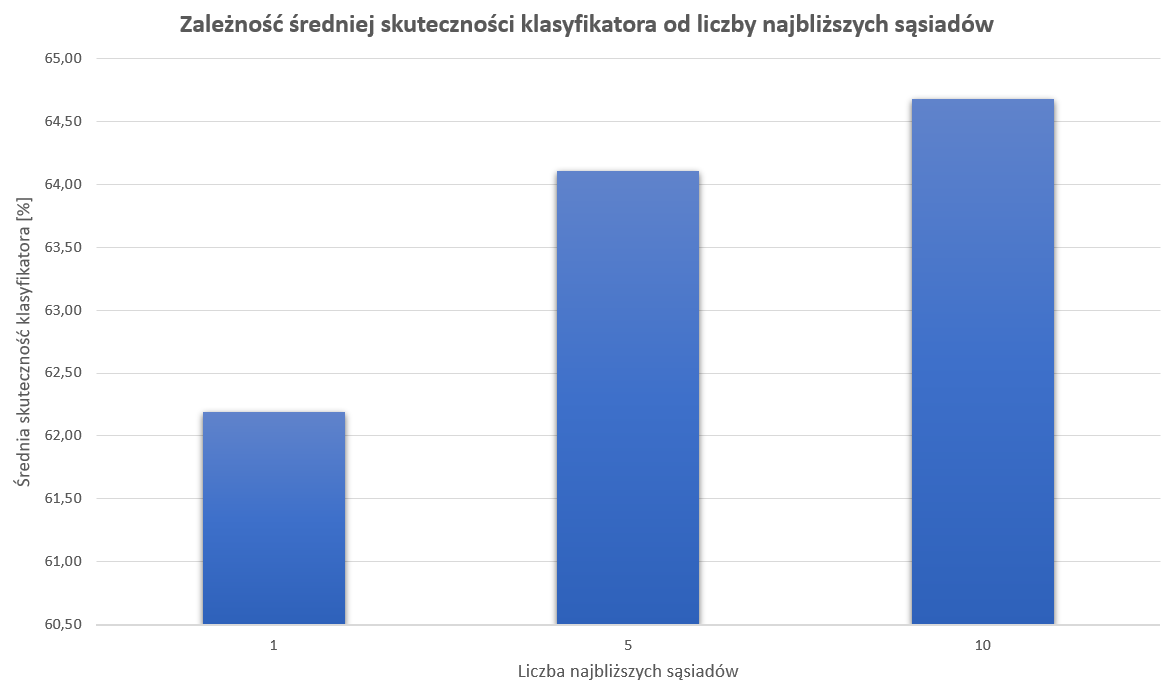
\includegraphics[width=16cm]{sasiedzi.png}
    \caption{Wykres zależności wyników klasyfikacji od liczby najbliższych sąsiadów.}
    \label{fig:sasiedzi}
\end{figure}

\noindent
Na podstawie wykresu przedstawionego na rysunku \ref{fig:sasiedzi} można wyciągnąć wniosek, że wzrost liczby najbliższych sąsiadów pozytywnie wpływa na wyniki klasyfikacji. Istnieje pewne prawdopodobieństwo, że dalsze zwiększanie wartości tego parametru mogłoby dodatkowo poprawić jej wyniki.

\newpage

\section{Wnioski}
Na podstawie wykonanych badań oraz analizy ich wyników wyłoniony został zestaw cech, które pozwalają na uzyskanie najwyżej ze statystycznego punktu widzenia skuteczności klasyfikatora KNN dla problemu diagnozowania zawałów:
\begin{itemize}
    \item Metryka obliczania odległości między sąsiadami - miara Manhattan.
    \item Liczba najistotniejszych cech z rankingu cech - 28.
    \item Liczba sąsiadów - 10.
\end{itemize}
Przedstawiony zestaw parametrów umożliwił uzyskanie średniej skuteczności na poziomie 72,2\%. Najwyższa skuteczność uzyskana w procedurze testowej wyniosła jednak 72,36\%, ale rezultat ten został uznany za mniej pewny na podstawie wyników testu t-Studenta. Algorytm KNN umożliwił rozwiązanie problemu diagnozowania zawałów u chorych z całkiem wysoką skutecznością.\\

Bardzo ważnym okazał się wybór metryki obliczania odległości między poszczególnymi sąsiadami. Metryka miejska pozwoliła uzyskać znacznie wyższą skuteczność klasyfikacji w porównaniu do metryki euklidesowej.\\

Wybór liczby najbliższych sąsiadów również miał zauważalny wpływ na jakość klasyfikacji, wzrost liczby sąsiadów skutkował wzrostem skuteczności działania klasyfikatora. W przyszłości warto byłoby przeprowadzić badania dla wyższych wartości tego parametru.\\

Liczba najlepszych cech z rankingu, branych pod uwagę w procesie klasyfikacji również wpływa na wyniki działania algorytmu, ale jest to wpływ zauważalnie niższy, niż w przypakdu pozostałych parametrów. Wybór liczby cech z zakresu od 12 do 35 pozwolił na uzyskanie podobnych wyników, jednak najlepsze wyniki zarejestrowano dla około 28 cech.

\newpage

\begin{thebibliography}{}
\bibitem{feature-select}\textit{https://towardsdatascience.com/feature-selection-correlation-and-p-value-da8921bfb3cf}, Selekcja cech - korelacja i współczynnik p.
\bibitem{feature-select-sklearn}\textit{https://towardsdatascience.com/feature-selection-with-pandas-e3690ad8504b}, Selekcja cech w bibliotece \texttt{scikit-learn}.
\bibitem{knn-lecture}\textit{http://home.agh.edu.pl/~horzyk/lectures/miw/KNN.pdf}, Metody Inteligencji Obliczeniowej - Metoda K Najbliższych Sąsiadów (KNN), Adrian Horzyk.
\bibitem{knn}\textit{http://enroute.pl/knn-klasyfikacja/}, Informacje o sposobie działania algorytmu KNN.
\bibitem{feature-selection-right}\textit{http://thatdatatho.com/2018/10/04/cross-validation-the-wrong-way-right-way-feature-selection/}, Walidacja krzyżowa z wyborem cech - poprawnie i nie poprawnie.
\bibitem{cross-valid-sklearn}\textit{https://scikit-learn.org/stable/auto\_examples/model\_selection/plot\_cv\_indices.html}, Wizualizacja zachowania walidacji krzyżowej w bibliotece \texttt{scikit-learn}.
\bibitem{metrics}\textit{https://scikit-learn.org/stable/modules/generated/sklearn.neighbors.DistanceMetric.html}, Informacje o dostępnych metrykach w dokumentacji biblioteki \texttt{scikit-learn}.
\bibitem{conf-matrix}\textit{https://scikit-learn.org/stable/modules/generated/sklearn.metrics.confusion\_matrix.html}, Dokumentacja sposobu generowania macierzy pomyłek z wykorzystaniem biblioteki scikit-learn.
\bibitem{sklearn}\textit{https://scikit-learn.org/stable/index.html}, Dokumentacja biblioteki \texttt{scikit-learn}.
\bibitem{t-student}\textit{Dealing with the evaluation of supervised classification algorithms}, Guzmán Santafé, Iñaki Inza, Jose Lozano, 2015.
\end{thebibliography}
\end{document}
